\documentclass[../main.tex]{subfiles}
\usepackage{silence}
\WarningFilter{glossaries}{No \printglossary or \printglossaries found}
\robExtConfigure{
    disable externalization,
    set placeholder eval={__LRPBARWIDTH__}{\lenToCm{0.25\baselineskip}},
    set placeholder eval={__LRPHEIGHT__}{\lenToCm{11\baselineskip}},
    set placeholder eval={__LRPWIDTH__}{\lenToCm{1.1\linewidth}},
    }
\begin{document}
\ifSubfilesClassLoaded{%
    \graphicspath{{figures/5-CrossAttOmics/}}%
    \setcounter{chapter}{4}%
}{
    \graphicspath{{../figures/5-CrossAttOmics/}}%
}
\chapter{CrossAttOmics}\label{chap:crossattomics}
\minitocpage

\section{Model Architecture}
 Our proposed architecture consists of two main components, illustrated in~\cref{fig:crossattomics_arch}.
 Initially, a series of encoders independently projects each modality into a representational space, utilizing a self-attention mechanism to capture intra-modality interactions.
 Subsequently, the architecture employs cross-attention modules to represent modality pairs, focusing on inter-modality interactions.
 Given the high dimensionality of omics data, direct computation of attention matrices becomes impractical.
 To address this challenge, we used a strategy of data decomposition into groups, effectively reducing the memory demands associated with attention calculations~\cite{AttOmics}.

 \begin{figure}[htbp]
    \begin{subcaptiongroup}
        \ifSubfilesClassLoaded{%
            \begin{spacing}{1}
    \fontsize{10}{10}\selectfont
    \mathversion{smaller}
    \begin{tikzpicture}<disable externalization>
        \node (a_lgd) [inner sep=0pt, anchor=south west] at (-1.3,0.4) {\textbf{A}};
        \node (b_lgd) [right=13.1cm of a_lgd.east, anchor=west, inner sep=0pt] {\textbf{B}};
        \node (c_lgd) [below=5.3cm of a_lgd.south, anchor=north, inner sep=0pt] {\textbf{C}};
        \node (d_lgd) [right=7.5cm of c_lgd.east, anchor=west, inner sep=0pt ] {\textbf{D}};
        \node (in_A) at (-1,0) [inner sep=1pt, text=mod1] {\(X^A\)};
        \node (in_C) [below=1.25cm of in_A.south, anchor=north, inner sep=1pt, text=mod3] {\(X^C\)};
        \node (in_B) [below=1.25cm of in_C.south, anchor=north, inner sep=1pt, text=mod2] {\(X^B\)};

        \foreach \lab/\c in {A/mod1, B/mod2, C/mod3}
            {
                \node (enc_\lab) [draw=\c, text=\c, thick, rounded rectangle, rounded rectangle west arc=none, right=3mm of in_\lab.east, anchor=west] {$\enc^{\lab}$};
                \node [text=\c, right=4mm of enc_\lab.north east, anchor=north west, inner sep=0pt, yshift=1mm] {\(U^{\lab}\)};
                \draw[thick, -stealth, color=\c] (in_\lab.east) -- (enc_\lab.west);
            }

        \begin{scope}[yshift=-6.2cm, scale=0.9, transform shape, every node/.style={font=\tiny, thick}]
            % \tikzstyle{every node}=[font=\tiny]
            \node (g1) [draw=mod2, square, inner sep=0pt, fill=mod2!10, text=mod2D] at (0,0) {$X^{B}_{g_1}$};
            \node (gi) [draw=mod2, square, below=0.5 cm of g1.south, anchor=north, inner sep=0pt, fill=mod2!10, text=mod2D] {$X^{B}_{g_j}$};
            \node (gk) [draw=mod2, square, below=0.5 cm of gi.south, anchor=north, inner sep=0pt, fill=mod2!10, text=mod2D] {$X^{B}_{g_k}$};

            \path (g1.south) -- (gi.north) node[midway, inner sep=0pt, yshift=1mm] () {$\vdots$};
            \path (gi.south) -- (gk.north) node[midway, inner sep=0pt, yshift=1mm] (dots) {$\vdots$};
            % \node (dots) [below=2mm of gi.south, anchor=center] {$\vdots$};

            \node (in_vec) [draw=mod2, rectangle, fit={(g1) (gi) (gk)}, left=3mm of g1.north west, anchor=north east, inner sep=0pt, fill=mod2!10, text=mod2D] {$X^B$};

            \draw [-stealth, color=mod2] (g1-|in_vec.east) -- (g1.west);
            \draw [-stealth, color=mod2] (gi-|in_vec.east) -- (gi.west);
            \draw [-stealth, color=mod2] (gk-|in_vec.east) -- (gk.west);

            \node (fcn1) [draw=mod2, rounded corners=3, right=3mm of g1.east, anchor=west, fill=mod2!10, text=mod2D, minimum height=4mm] {\hyperref[eq:attomics_groups_proj]{FCN}};
            \node (fcni) [draw=mod2, rounded corners=3, right=3mm of gi.east, anchor=west, fill=mod2!10, text=mod2D, minimum height=4mm] {\hyperref[eq:attomics_groups_proj]{FCN}};
            \node (fcnk) [draw=mod2, rounded corners=3, right=3mm of gk.east, anchor=west, fill=mod2!10, text=mod2D, minimum height=4mm] {\hyperref[eq:attomics_groups_proj]{FCN}};

            \draw [-stealth, color=mod2] (g1.east) -- (fcn1.west);
            \draw [-stealth, color=mod2] (gi.east) -- (fcni.west);
            \draw [-stealth, color=mod2] (gk.east) -- (fcnk.west);

            \node (g1p) [draw=mod2, square, right=0.3 cm of fcn1.east, anchor=west, inner sep=0pt, fill=mod2!10, text=mod2D] {$X^{'B}_{g_1}$};
            \node (gip) [draw=mod2, square, right=0.3 cm of fcni.east, anchor=west, inner sep=0pt, fill=mod2!10, text=mod2D] {$X^{'B}_{g_j}$};
            \node (gkp) [draw=mod2, square, right=0.3 cm of fcnk.east, anchor=west, inner sep=0pt, fill=mod2!10, text=mod2D] {$X^{'B}_{g_k}$};

            \draw [-stealth, color=mod2] (fcn1.east) -- (g1p.west);
            \draw [-stealth, color=mod2] (fcni.east) -- (gip.west);
            \draw [-stealth, color=mod2] (fcnk.east) -- (gkp.west);

            \path (g1p.south) -- (gip.north) node[midway, draw=mod2, square, inner sep=0pt, xshift=8mm, anchor=west, fill=mod2!10, text=mod2D] (mhsa_gj) {$X^{'B}_{g_j}$};
            \path (gip.south) -- (gkp.north) node[midway, draw=mod2, square, inner sep=0pt, xshift=8mm, anchor=west, fill=mod2!10, text=mod2D] (mhsa_G) {\hyperref[eq:attomics_groups_proj]{$X^{'B}_{G}$}};

            \node (Q) [draw=mod2, square, right=15mm of g1p.east, anchor=west, inner sep=0pt, fill=mod2!10, text=mod2D] {$Q_{g_j}$};
            \node (K) [draw=mod2, square, right=15mm of gip.east, anchor=west, fill=mod2!10, text=mod2D] {K};
            \node (V) [draw=mod2, square, right=15mm of gkp.east, anchor=west, fill=mod2!10, text=mod2D] {V};

            \draw[-stealth, color=mod2, rounded corners=3] (mhsa_gj) |- (Q);
            \draw[-stealth, color=mod2, rounded corners=3] (mhsa_G) |- (K);
            \draw[-stealth, color=mod2, rounded corners=3] (mhsa_G) |- (V);

            \node (A) [draw=mod2, rectangle, fit={(Q) (K)}, right=4mm of K.south east, anchor=south west, inner sep=0pt, fill=mod2!10, text=mod2D] {$A^{B}_{g_j}$};
            \node (out) [draw=mod2, square, right=1.2cm of V.east, anchor=west, fill=mod2!10, text=mod2D] {};
            \draw[-stealth, color=mod2] (Q) -- (Q-|A.west);
            \draw[-stealth, color=mod2] (K) -- (K-|A.west);
            \draw[-stealth, color=mod2] (V) -- (out);
            \draw[-stealth, color=mod2, rounded corners=3] (A) -| (out);
            \node (mhsa) [draw, fit={(Q) (K) (V) (out) (mhsa_gj) (mhsa_G)}, dashed, rounded corners=5, inner xsep=2pt, inner ysep=3mm] {};
            \node [left=1mm of mhsa.north east, anchor=north east, inner sep=1pt, yshift=-0.5mm] {MHSA};
            \node [right=1mm of mhsa.north west, anchor=north west, inner sep=1pt, yshift=-0.5mm] {\cref{eq:enc_mhsa}};
            % \draw[-stealth] (out) -- (out-|mhsa.east);
            \draw[-stealth, color=mod2] (g1p) -- (g1p-|mhsa.west);
            \draw[-stealth, color=mod2] (gip) -- (gip-|mhsa.west);
            \draw[-stealth, color=mod2] (gkp) -- (gkp-|mhsa.west);
            \node (outk) [draw=mod2, square, right=4cm of gkp.east, anchor=west, inner sep=0pt, fill=mod2!10, text=mod2D] {$U^B_{g_k}$};
            \node (outi) [draw=mod2, square, inner sep=0pt, fill=mod2!10, text=mod2D] at (gip -| outk) {$U^B_{g_j}$};
            \node (out1) [draw=mod2, square, inner sep=0pt, fill=mod2!10, text=mod2D] at (g1p -| outk) {$U^B_{g_1}$};

            \draw[-stealth, color=mod2] (outk-|mhsa.east) -- (outk);
            \draw[-stealth, color=mod2] (outi-|mhsa.east) -- (outi);
            \draw[-stealth, color=mod2] (out1-|mhsa.east) -- (out1);
        \end{scope}

        \begin{scope}[xshift=6.8cm, yshift=-5.7cm, scale=0.9, transform shape, every node/.style={font=\tiny, thick}]
            \node (b1) [draw=mod1, fill=mod1!10, square, inner sep=0pt, minimum size=10mm] at (0,0) {};
            \node (b2) [draw=mod1, fill=mod1!10, square, right=0mm of b1.east, anchor=west, inner sep=0pt, minimum size=10mm, xshift=-0.8pt] {};
            \node (b3) [draw=mod1, fill=mod1!10, square, right=0mm of b2.east, anchor=west, inner sep=0pt, minimum size=10mm, xshift=-0.8pt] {};
            \node [text=mod1D] at (b2.center) {\(U^{j}_{g_p}\)};

            \node (a1) [draw=mod2, fill=mod2!10, square, below=5mm of b2.south, anchor=north, inner sep=0pt, minimum size=10mm] {};
            \node (a2) [draw=mod2, fill=mod2!10, square, below=0mm of a1.south, anchor=north, inner sep=0pt, minimum size=10mm, yshift=0.8pt] {};
            \node (a3) [draw=mod2, fill=mod2!10, square, below=0mm of a2.south, anchor=north, inner sep=0pt, minimum size=10mm, yshift=0.8pt] {};
            \node (a4) [draw=mod2, fill=mod2!10, square, below=0mm of a3.south, anchor=north, inner sep=0pt, minimum size=10mm, yshift=0.8pt] {};
            \node [text=mod2D] at (a4.center) {\(U^{i}_{g_{k^i}}\)};

            \node (q1) [draw=mod1, fill=mod1!10, square, right=6mm of b3.east, anchor=west, inner sep=0pt, minimum size=10mm] {};
            \node (q2) [draw=mod1, fill=mod1!10, square, right=0mm of q1.east, anchor=west, inner sep=0pt, minimum size=10mm, xshift=-0.8pt] {};
            \node (q3) [draw=mod1, fill=mod1!10, square, right=0mm of q2.east, anchor=west, inner sep=0pt, minimum size=10mm, xshift=-0.8pt] {};
            \node [text=mod1D] at (q2.center) {\(Q^{j}_{g_p}\)};

            \node (k3) [draw=mod2, fill=mod2!10, square, inner sep=0pt, minimum size=10mm, anchor=west] at (a1.east-|q2) {};
            \node (k2) [draw=mod2, fill=mod2!10, square, left=0mm of k3.west, anchor=east, inner sep=0pt, minimum size=10mm, xshift=0.8pt] {};
            \node (k1) [draw=mod2, fill=mod2!10, square, left=0mm of k2.west, anchor=east, inner sep=0pt, minimum size=10mm, xshift=0.8pt] {};
            \node (k4) [draw=mod2, fill=mod2!10, square, right=0mm of k3.east, anchor=west, inner sep=0pt, minimum size=10mm, xshift=-0.8pt] {};
            \node [text=mod2D] at (k4.center) {\(K^{i}_{g_{k^i}}\)};

            \node (v3) [draw=mod2, fill=mod2!10, square, inner sep=0pt, minimum size=10mm, anchor=west] at (a4.east-|q2) {};
            \node (v2) [draw=mod2, fill=mod2!10, square, left=0mm of v3.west, anchor=east, inner sep=0pt, minimum size=10mm, xshift=0.8pt] {};
            \node (v1) [draw=mod2, fill=mod2!10, square, left=0mm of v2.west, anchor=east, inner sep=0pt, minimum size=10mm, xshift=0.8pt] {};
            \node (v4) [draw=mod2, fill=mod2!10, square, right=0mm of v3.east, anchor=west, inner sep=0pt, minimum size=10mm, xshift=-0.8pt] {};
            \node [text=mod2D] at (v4.center) {\(V^{i}_{g_{k^i}}\)};

            % Attention matrix
            \path (q3.south) -- (k3.north) coordinate [midway, draw=black!50, square, anchor=west,minimum size=7mm, xshift=12mm, inner color=mod2!60, outer color=mod1!80] (a21);
            \node (a11) [draw=black!50, yshift=-0.8pt, square, above=0mm of a21.north, anchor=south,minimum size=7mm, inner color=mod2!60, outer color=mod1!80] {};
            \node (a31) [draw=black!50, yshift=0.8pt, square, below=0mm of a21.south, anchor=north,minimum size=7mm, inner color=mod2!60, outer color=mod1!80] {};
            \foreach \col/\yi in {2/1,3/2,4/3}{
                    \node (a1\col) [draw=black!50, xshift=-0.8pt, square, right=0mm of a1\yi.east, anchor=west,minimum size=7mm, inner color=mod2!60, outer color=mod1!80] {};
                    \node (a2\col) [draw=black!50, xshift=-0.8pt, square, right=0mm of a2\yi.east, anchor=west,minimum size=7mm, inner color=mod2!60, outer color=mod1!80] {};
                    \node (a3\col) [draw=black!50, xshift=-0.8pt, square, right=0mm of a3\yi.east, anchor=west,minimum size=7mm, inner color=mod2!60, outer color=mod1!80] {};
                }

            \node (Aij) [draw=H, fit={(a21) (a22) (a23) (a24)}, dashed, rounded corners=5] {};
            \node [right=0mm of Aij.east, anchor=south west, inner sep=1pt, text=H] {\hyperref[eq:cross_att_weights]{\(A^{i\rightarrow j}_{g_p}\)}};
            \node [left=0mm of Aij.west, anchor=east, inner sep=1pt, text=H] {\cref{eq:cross_att_weights}};

            \node (o3) [draw=mod1, fill=mod1!10, square, inner sep=0pt, minimum size=10mm] at (v4-|a34.south) {};
            \node (o2) [draw=mod1, fill=mod1!10, square, above=0cm of o3.north, anchor=south, inner sep=0pt, minimum size=10mm, yshift=-0.8pt] {};
            \node (o1) [draw=mod1, fill=mod1!10, square, above=0mm of o2.north, anchor=south, inner sep=0pt, minimum size=10mm, yshift=-0.8pt] {};
            \node [inner sep=0pt, text=mod1D] at (o2.center) {\hyperref[eq:cross_att]{\(Z^{i\rightarrow j}_{g_p}\)}};

            \draw[-stealth, color=mod1] (b3) to ["\(W^{Q}\)"] (q1);
            \path (a1.east) -- (k1.west) coordinate [midway, inner sep=0pt, xshift=-3mm] (midk2);
            \node [above=0mm of midk2.north, anchor=south west, text=mod2] {\(W^{K}\)};
            \node (midk1) at (a2.south east -| midk2) {};
            \draw[-stealth, rounded corners=5, color=mod2] (a2.south east) -- (midk1.center) -- (midk2.center) -- (k1.west);

            \path (a4.east) -- (v1.west) coordinate [midway, inner sep=0pt, xshift=-3mm] (midv2);
            \node [below=0mm of midv2.north, anchor=north west, text=mod2] {\(W^{V}\)};
            \node (midv1) at (a2.south east -| midv2) {};
            \draw[-stealth, rounded corners=5, color=mod2] (a2.south east) -- (midv1.center) -- (midv2.center) -- (v1.west);

            \path (v4.east) -- (o3.west) coordinate [midway] (mido3);
            \node (mido2) at (mido3 |- o2) {};
            \draw[-stealth, rounded corners=5, color=mod2] (v4) -- (mido3.center) -- (mido2.center) -- (o2);
            \node (midAo3) at (a32.south east |- o2) {};
            \node [left=0mm of midAo3.west, anchor=south east, inner sep=1pt] {\cref{eq:cross_att}};
            \draw[-stealth, rounded corners=5, color=mod1] (a32.south east) -- ([yshift=2mm]midAo3.center) -- ([yshift=2mm]o2.west);

            \draw [-stealth, color=mod1] (q3.east |- a11) -- (a11);
            \draw [-stealth, color=mod2] (k4.east |- a31) -- (a31);

            \node (AijW) [above=1mm of a13.north east, anchor=south east, inner sep=0pt] {\hyperref[eq:cross_att_weight]{\( a^{i\rightarrow j}_{g_p,g_{k^i}}\)}};
            \draw[-stealth] (AijW.east) to[bend left] (a24.center);
        \end{scope}

        \path (enc_A.south) -- (enc_C.north) node[midway, rounded corners=5, anchor=center, xshift=2.7cm,top color=mod1,bottom color=mod3,text=white, font=\footnotesize] (cross_AC) {CrossAttention};
        \path (enc_C.south) -- (enc_B.north) node[midway, rounded corners=5, anchor=center, xshift=2.7cm,top color=mod3,bottom color=mod2,text=white, font=\footnotesize] (cross_BC) {CrossAttention};
        \path let \p1=(cross_AC.center), \p2=(cross_BC.center), \n1={veclen(\x2-\x1,\y2-\y1)} in node[below=\n1 of cross_BC.center, anchor=center, rounded corners=5,top color=mod2,bottom color=mod1,text=white, font=\footnotesize] (cross_AB) {CrossAttention};

        \draw [-stealth, thick, rounded corners=5, color=mod3] (enc_C.east) -| (cross_BC.north);
        \draw [-stealth, thick, rounded corners=5, color=mod3] (enc_C.east) -| (cross_AC.south);
        \draw [-stealth, thick, rounded corners=5, color=mod2] (enc_B.east) -| (cross_BC.south);
        \draw [-stealth, thick, rounded corners=5, color=mod2] (enc_B.east) -| (cross_AB.north);
        \draw [-stealth, thick, rounded corners=5, color=mod1] (enc_A.east) -| (cross_AC.north);
        \coordinate (xx1) at (enc_A.east -| cross_AC.west);
        \path (enc_A.east) -- (xx1) coordinate [midway, xshift=3mm] (mid1);
        \path let \p1=(enc_A.east), \p2=(cross_AB.south west), \p3=(cross_AC.north), \n1={veclen(\x1-\x1,\y2-\y1)}, \n2={4mm}, \n3={\n1 + \n2} in coordinate [below=\n3 of mid1] (mid2) coordinate [below=\n2 of cross_AB.south] (mid3);
        \draw [-stealth, thick, rounded corners=5, color=mod1] (enc_A.east) -- (mid1) -- (mid2) -- (mid3) -- (cross_AB.south);

        \foreach \t/\l/\c in {AC/A\rightarrow C/mod3, BC/B\rightarrow C/mod3, AB/A\rightarrow B/mod2} {
                \node (Z_\t) [inner sep=1pt, right=3mm of cross_\t.east, text=\c] {\(Z^{\l}\)};
                \draw[thick, -stealth, color=\c] (cross_\t.east) -- (Z_\t.west);
                \node at ([xshift=0.5ex, yshift=0.5em]cross_\t.north) [right, inner sep=0pt] {\tiny\ifthenelse{\equal{\t}{AC}}{\(K,V\)}{\(Q\)}};
                \node at ([xshift=0.5ex, yshift=-0.5em]cross_\t.south) [right, inner sep=0pt] {\tiny\ifthenelse{\equal{\t}{AC}}{\(Q\)}{\(K,V\)}};
            }

        \node (cat_C) [draw=mod3, thick, signal, right=5.35cm of enc_C.east, anchor=west, text height=0.5cm, text width=0.25cm] {};
        \node (cat_B) [draw=mod2, thick, signal, right=5.35cm of enc_B.east, anchor=west, text height=0.5cm, text width=0.25cm] {};
        \draw[thick, -stealth, color=mod3] (enc_C.east) -- (cat_C.west);
        \draw[thick, -stealth, color=mod2] (enc_B.east) -- (cat_B.west);

        \path let \p1=(Z_AC.east), \p2=(cat_C.west), \n1={veclen(\x2-\x1,\y1-\y1)/2} in coordinate [right=\n1 of Z_AC.east] (cat_ac) coordinate [right=\n1 of Z_BC.east] (cat_bc) coordinate [left=\n1 of cat_C.west, yshift=2mm] (cat_ac2) coordinate [left=\n1 of cat_C.west, yshift=-2mm] (cat_bc2) coordinate [right=\n1 of Z_AB.east] (cat_ab) coordinate [left=\n1 of cat_B.west, yshift=-2mm] (cat_ab2);
        \draw[thick, -stealth, rounded corners=5pt, color=mod3] (Z_AC.east) -- (cat_ac) -- (cat_ac2) -- ([yshift=2mm]cat_C.west);
        \draw[thick, -stealth, rounded corners=5pt, color=mod3] (Z_BC.east) -- (cat_bc) -- (cat_bc2) -- ([yshift=-2mm]cat_C.west);
        \draw[thick, -stealth, rounded corners=5pt, color=mod2] (Z_AB.east) -- (cat_ab) -- (cat_ab2) -- ([yshift=-2mm]cat_B.west);

        \foreach \t/\c in {B/mod2, C/mod3} {
                \node (Z_\t) [inner sep=1pt, right=2mm of cat_\t.east, text=\c] {\(Z^{\t}\)};
                \node (sa_\t) [right=2mm of Z_\t.east, draw=\c, thick, rounded corners=5, font=\footnotesize] {MHSA};
                \node (Z_\t2) [inner sep=1pt, right=2mm of sa_\t.east, text=\c] {\(Z^{\t}\)};
                \draw[thick, -stealth, color=\c] (cat_\t.east) -- (Z_\t.west) ;
                \draw[thick, -stealth, color=\c] (Z_\t.east) -- (sa_\t.west) ;
                \draw[thick, -stealth, color=\c] (sa_\t.east) -- (Z_\t2.west) ;
            }
        \path[name path=ac] (in_A.east)--([xshift=14cm]in_A.east);
        \path[name path=bd] (Z_C2.north)--([yshift=2.5cm]Z_C2.north);
        \path [name intersections={of=ac and bd,by=E}];
        \node (Z_A) at (E) [inner sep=1pt, text=mod1] {\(Z^A\)};
        \draw[thick, -stealth, color=mod1] (enc_A.east) -- (Z_A.west) ;

        \node (cat) [draw, thick, signal, right=.6cm of Z_C2.east, anchor=west, text height=0.5cm, text width=0.25cm] {};
        \draw[thick, -stealth, color=mod3] (Z_C2.east) -- (cat.west) ;
        \path let \p1=(Z_A.east), \p2=(cat.west), \n1={veclen(\x2-\x1,\y1-\y1)/2} in coordinate [right=\n1 of Z_A.east] (cat_za) coordinate [right=\n1 of Z_B2.east] (cat_zb) coordinate [left=\n1 of cat.west, yshift=2mm] (cat_za2) coordinate [left=\n1 of cat.west, yshift=-2mm] (cat_zb2);
        \draw[thick, -stealth, rounded corners=5, color=mod1] (Z_A.east) -- (cat_za) -- (cat_za2) -- ([yshift=2mm]cat.west) ;
        \draw[thick, -stealth, rounded corners=5, color=mod2] (Z_B2.east) -- (cat_zb) -- (cat_zb2) -- ([yshift=-2mm]cat.west) ;

        \node (Z) [right=3mm of cat.east, inner sep=1pt] {\(Z\)};
        \node (FCN) [draw, thick, rounded corners=5, right=3mm of Z.east, anchor=west, font=\footnotesize] {FCN};
        \node (out) [inner sep=1pt, right=3mm of FCN.east, anchor=west] {\(\hat{Y}\)};
        \draw [thick, -stealth] (cat.east) -- (Z.west);
        \draw [thick, -stealth] (Z.east) -- (FCN.west);
        \draw [thick, -stealth] (FCN.east) -- (out.west);

        \node (A) [inner sep=1pt, right=2.5cm of Z_A.east, anchor=west, text=mod1, yshift=2mm] {A};
        \node (B) [inner sep=1pt, right=6mm of A.east, anchor=west, text=mod2] {B};
        \node (C) [inner sep=1pt, below=6mm of B.south, anchor=north, text=mod3] {C};
        \draw[thick, -stealth] (A.east) -- (B.west) ;
        \draw[thick, -stealth] (B.south) -- (C.north) ;
        \draw[thick, -stealth, rounded corners=5] (A.south) |- (C.west) ;

        \node (cat_lgd) [draw, thick, signal, below=3mm of cat.south west, anchor=north west, text height=0.5cm, text width=0.25cm] {};
        %\path let \p1=(cat_lgd.east), \p2=(cat_lgd.west), \n1={veclen(\x2-\x1,\y2-\y1)} in node (opt_lgd) [draw, thick, rounded corners=5, dashed, below=5mm of cat_lgd.south west, anchor=north west, text height=0.2cm, minimum width=\n1] {};
        \node [right=1mm of cat_lgd.east, anchor=west] {Concatenate};
        %\node [right=1mm of opt_lgd.east, anchor=west] {Optionnal};

        \begin{scope}[on background layer={color=black!8}]
            \node [fill, fit={(A) (B) (C) (b_lgd)}] {}; %fit margins={bottom=10pt,top=0pt},
        \end{scope}

    \end{tikzpicture}
    \mathversion{normal}
\end{spacing}

%
        }{
            \begin{spacing}{1}
    \fontsize{10}{10}\selectfont
    \mathversion{smaller}
    \begin{tikzpicture}<disable externalization>
        \node (a_lgd) [inner sep=0pt, anchor=south west] at (-1.3,0.4) {\textbf{A}};
        \node (b_lgd) [right=13.1cm of a_lgd.east, anchor=west, inner sep=0pt] {\textbf{B}};
        \node (c_lgd) [below=5.3cm of a_lgd.south, anchor=north, inner sep=0pt] {\textbf{C}};
        \node (d_lgd) [right=7.5cm of c_lgd.east, anchor=west, inner sep=0pt ] {\textbf{D}};
        \node (in_A) at (-1,0) [inner sep=1pt, text=mod1] {\(X^A\)};
        \node (in_C) [below=1.25cm of in_A.south, anchor=north, inner sep=1pt, text=mod3] {\(X^C\)};
        \node (in_B) [below=1.25cm of in_C.south, anchor=north, inner sep=1pt, text=mod2] {\(X^B\)};

        \foreach \lab/\c in {A/mod1, B/mod2, C/mod3}
            {
                \node (enc_\lab) [draw=\c, text=\c, thick, rounded rectangle, rounded rectangle west arc=none, right=3mm of in_\lab.east, anchor=west] {$\enc^{\lab}$};
                \node [text=\c, right=4mm of enc_\lab.north east, anchor=north west, inner sep=0pt, yshift=1mm] {\(U^{\lab}\)};
                \draw[thick, -stealth, color=\c] (in_\lab.east) -- (enc_\lab.west);
            }

        \begin{scope}[yshift=-6.2cm, scale=0.9, transform shape, every node/.style={font=\tiny, thick}]
            % \tikzstyle{every node}=[font=\tiny]
            \node (g1) [draw=mod2, square, inner sep=0pt, fill=mod2!10, text=mod2D] at (0,0) {$X^{B}_{g_1}$};
            \node (gi) [draw=mod2, square, below=0.5 cm of g1.south, anchor=north, inner sep=0pt, fill=mod2!10, text=mod2D] {$X^{B}_{g_j}$};
            \node (gk) [draw=mod2, square, below=0.5 cm of gi.south, anchor=north, inner sep=0pt, fill=mod2!10, text=mod2D] {$X^{B}_{g_k}$};

            \path (g1.south) -- (gi.north) node[midway, inner sep=0pt, yshift=1mm] () {$\vdots$};
            \path (gi.south) -- (gk.north) node[midway, inner sep=0pt, yshift=1mm] (dots) {$\vdots$};
            % \node (dots) [below=2mm of gi.south, anchor=center] {$\vdots$};

            \node (in_vec) [draw=mod2, rectangle, fit={(g1) (gi) (gk)}, left=3mm of g1.north west, anchor=north east, inner sep=0pt, fill=mod2!10, text=mod2D] {$X^B$};

            \draw [-stealth, color=mod2] (g1-|in_vec.east) -- (g1.west);
            \draw [-stealth, color=mod2] (gi-|in_vec.east) -- (gi.west);
            \draw [-stealth, color=mod2] (gk-|in_vec.east) -- (gk.west);

            \node (fcn1) [draw=mod2, rounded corners=3, right=3mm of g1.east, anchor=west, fill=mod2!10, text=mod2D, minimum height=4mm] {\hyperref[eq:attomics_groups_proj]{FCN}};
            \node (fcni) [draw=mod2, rounded corners=3, right=3mm of gi.east, anchor=west, fill=mod2!10, text=mod2D, minimum height=4mm] {\hyperref[eq:attomics_groups_proj]{FCN}};
            \node (fcnk) [draw=mod2, rounded corners=3, right=3mm of gk.east, anchor=west, fill=mod2!10, text=mod2D, minimum height=4mm] {\hyperref[eq:attomics_groups_proj]{FCN}};

            \draw [-stealth, color=mod2] (g1.east) -- (fcn1.west);
            \draw [-stealth, color=mod2] (gi.east) -- (fcni.west);
            \draw [-stealth, color=mod2] (gk.east) -- (fcnk.west);

            \node (g1p) [draw=mod2, square, right=0.3 cm of fcn1.east, anchor=west, inner sep=0pt, fill=mod2!10, text=mod2D] {$X^{'B}_{g_1}$};
            \node (gip) [draw=mod2, square, right=0.3 cm of fcni.east, anchor=west, inner sep=0pt, fill=mod2!10, text=mod2D] {$X^{'B}_{g_j}$};
            \node (gkp) [draw=mod2, square, right=0.3 cm of fcnk.east, anchor=west, inner sep=0pt, fill=mod2!10, text=mod2D] {$X^{'B}_{g_k}$};

            \draw [-stealth, color=mod2] (fcn1.east) -- (g1p.west);
            \draw [-stealth, color=mod2] (fcni.east) -- (gip.west);
            \draw [-stealth, color=mod2] (fcnk.east) -- (gkp.west);

            \path (g1p.south) -- (gip.north) node[midway, draw=mod2, square, inner sep=0pt, xshift=8mm, anchor=west, fill=mod2!10, text=mod2D] (mhsa_gj) {$X^{'B}_{g_j}$};
            \path (gip.south) -- (gkp.north) node[midway, draw=mod2, square, inner sep=0pt, xshift=8mm, anchor=west, fill=mod2!10, text=mod2D] (mhsa_G) {\hyperref[eq:attomics_groups_proj]{$X^{'B}_{G}$}};

            \node (Q) [draw=mod2, square, right=15mm of g1p.east, anchor=west, inner sep=0pt, fill=mod2!10, text=mod2D] {$Q_{g_j}$};
            \node (K) [draw=mod2, square, right=15mm of gip.east, anchor=west, fill=mod2!10, text=mod2D] {K};
            \node (V) [draw=mod2, square, right=15mm of gkp.east, anchor=west, fill=mod2!10, text=mod2D] {V};

            \draw[-stealth, color=mod2, rounded corners=3] (mhsa_gj) |- (Q);
            \draw[-stealth, color=mod2, rounded corners=3] (mhsa_G) |- (K);
            \draw[-stealth, color=mod2, rounded corners=3] (mhsa_G) |- (V);

            \node (A) [draw=mod2, rectangle, fit={(Q) (K)}, right=4mm of K.south east, anchor=south west, inner sep=0pt, fill=mod2!10, text=mod2D] {$A^{B}_{g_j}$};
            \node (out) [draw=mod2, square, right=1.2cm of V.east, anchor=west, fill=mod2!10, text=mod2D] {};
            \draw[-stealth, color=mod2] (Q) -- (Q-|A.west);
            \draw[-stealth, color=mod2] (K) -- (K-|A.west);
            \draw[-stealth, color=mod2] (V) -- (out);
            \draw[-stealth, color=mod2, rounded corners=3] (A) -| (out);
            \node (mhsa) [draw, fit={(Q) (K) (V) (out) (mhsa_gj) (mhsa_G)}, dashed, rounded corners=5, inner xsep=2pt, inner ysep=3mm] {};
            \node [left=1mm of mhsa.north east, anchor=north east, inner sep=1pt, yshift=-0.5mm] {MHSA};
            \node [right=1mm of mhsa.north west, anchor=north west, inner sep=1pt, yshift=-0.5mm] {\cref{eq:enc_mhsa}};
            % \draw[-stealth] (out) -- (out-|mhsa.east);
            \draw[-stealth, color=mod2] (g1p) -- (g1p-|mhsa.west);
            \draw[-stealth, color=mod2] (gip) -- (gip-|mhsa.west);
            \draw[-stealth, color=mod2] (gkp) -- (gkp-|mhsa.west);
            \node (outk) [draw=mod2, square, right=4cm of gkp.east, anchor=west, inner sep=0pt, fill=mod2!10, text=mod2D] {$U^B_{g_k}$};
            \node (outi) [draw=mod2, square, inner sep=0pt, fill=mod2!10, text=mod2D] at (gip -| outk) {$U^B_{g_j}$};
            \node (out1) [draw=mod2, square, inner sep=0pt, fill=mod2!10, text=mod2D] at (g1p -| outk) {$U^B_{g_1}$};

            \draw[-stealth, color=mod2] (outk-|mhsa.east) -- (outk);
            \draw[-stealth, color=mod2] (outi-|mhsa.east) -- (outi);
            \draw[-stealth, color=mod2] (out1-|mhsa.east) -- (out1);
        \end{scope}

        \begin{scope}[xshift=6.8cm, yshift=-5.7cm, scale=0.9, transform shape, every node/.style={font=\tiny, thick}]
            \node (b1) [draw=mod1, fill=mod1!10, square, inner sep=0pt, minimum size=10mm] at (0,0) {};
            \node (b2) [draw=mod1, fill=mod1!10, square, right=0mm of b1.east, anchor=west, inner sep=0pt, minimum size=10mm, xshift=-0.8pt] {};
            \node (b3) [draw=mod1, fill=mod1!10, square, right=0mm of b2.east, anchor=west, inner sep=0pt, minimum size=10mm, xshift=-0.8pt] {};
            \node [text=mod1D] at (b2.center) {\(U^{j}_{g_p}\)};

            \node (a1) [draw=mod2, fill=mod2!10, square, below=5mm of b2.south, anchor=north, inner sep=0pt, minimum size=10mm] {};
            \node (a2) [draw=mod2, fill=mod2!10, square, below=0mm of a1.south, anchor=north, inner sep=0pt, minimum size=10mm, yshift=0.8pt] {};
            \node (a3) [draw=mod2, fill=mod2!10, square, below=0mm of a2.south, anchor=north, inner sep=0pt, minimum size=10mm, yshift=0.8pt] {};
            \node (a4) [draw=mod2, fill=mod2!10, square, below=0mm of a3.south, anchor=north, inner sep=0pt, minimum size=10mm, yshift=0.8pt] {};
            \node [text=mod2D] at (a4.center) {\(U^{i}_{g_{k^i}}\)};

            \node (q1) [draw=mod1, fill=mod1!10, square, right=6mm of b3.east, anchor=west, inner sep=0pt, minimum size=10mm] {};
            \node (q2) [draw=mod1, fill=mod1!10, square, right=0mm of q1.east, anchor=west, inner sep=0pt, minimum size=10mm, xshift=-0.8pt] {};
            \node (q3) [draw=mod1, fill=mod1!10, square, right=0mm of q2.east, anchor=west, inner sep=0pt, minimum size=10mm, xshift=-0.8pt] {};
            \node [text=mod1D] at (q2.center) {\(Q^{j}_{g_p}\)};

            \node (k3) [draw=mod2, fill=mod2!10, square, inner sep=0pt, minimum size=10mm, anchor=west] at (a1.east-|q2) {};
            \node (k2) [draw=mod2, fill=mod2!10, square, left=0mm of k3.west, anchor=east, inner sep=0pt, minimum size=10mm, xshift=0.8pt] {};
            \node (k1) [draw=mod2, fill=mod2!10, square, left=0mm of k2.west, anchor=east, inner sep=0pt, minimum size=10mm, xshift=0.8pt] {};
            \node (k4) [draw=mod2, fill=mod2!10, square, right=0mm of k3.east, anchor=west, inner sep=0pt, minimum size=10mm, xshift=-0.8pt] {};
            \node [text=mod2D] at (k4.center) {\(K^{i}_{g_{k^i}}\)};

            \node (v3) [draw=mod2, fill=mod2!10, square, inner sep=0pt, minimum size=10mm, anchor=west] at (a4.east-|q2) {};
            \node (v2) [draw=mod2, fill=mod2!10, square, left=0mm of v3.west, anchor=east, inner sep=0pt, minimum size=10mm, xshift=0.8pt] {};
            \node (v1) [draw=mod2, fill=mod2!10, square, left=0mm of v2.west, anchor=east, inner sep=0pt, minimum size=10mm, xshift=0.8pt] {};
            \node (v4) [draw=mod2, fill=mod2!10, square, right=0mm of v3.east, anchor=west, inner sep=0pt, minimum size=10mm, xshift=-0.8pt] {};
            \node [text=mod2D] at (v4.center) {\(V^{i}_{g_{k^i}}\)};

            % Attention matrix
            \path (q3.south) -- (k3.north) coordinate [midway, draw=black!50, square, anchor=west,minimum size=7mm, xshift=12mm, inner color=mod2!60, outer color=mod1!80] (a21);
            \node (a11) [draw=black!50, yshift=-0.8pt, square, above=0mm of a21.north, anchor=south,minimum size=7mm, inner color=mod2!60, outer color=mod1!80] {};
            \node (a31) [draw=black!50, yshift=0.8pt, square, below=0mm of a21.south, anchor=north,minimum size=7mm, inner color=mod2!60, outer color=mod1!80] {};
            \foreach \col/\yi in {2/1,3/2,4/3}{
                    \node (a1\col) [draw=black!50, xshift=-0.8pt, square, right=0mm of a1\yi.east, anchor=west,minimum size=7mm, inner color=mod2!60, outer color=mod1!80] {};
                    \node (a2\col) [draw=black!50, xshift=-0.8pt, square, right=0mm of a2\yi.east, anchor=west,minimum size=7mm, inner color=mod2!60, outer color=mod1!80] {};
                    \node (a3\col) [draw=black!50, xshift=-0.8pt, square, right=0mm of a3\yi.east, anchor=west,minimum size=7mm, inner color=mod2!60, outer color=mod1!80] {};
                }

            \node (Aij) [draw=H, fit={(a21) (a22) (a23) (a24)}, dashed, rounded corners=5] {};
            \node [right=0mm of Aij.east, anchor=south west, inner sep=1pt, text=H] {\hyperref[eq:cross_att_weights]{\(A^{i\rightarrow j}_{g_p}\)}};
            \node [left=0mm of Aij.west, anchor=east, inner sep=1pt, text=H] {\cref{eq:cross_att_weights}};

            \node (o3) [draw=mod1, fill=mod1!10, square, inner sep=0pt, minimum size=10mm] at (v4-|a34.south) {};
            \node (o2) [draw=mod1, fill=mod1!10, square, above=0cm of o3.north, anchor=south, inner sep=0pt, minimum size=10mm, yshift=-0.8pt] {};
            \node (o1) [draw=mod1, fill=mod1!10, square, above=0mm of o2.north, anchor=south, inner sep=0pt, minimum size=10mm, yshift=-0.8pt] {};
            \node [inner sep=0pt, text=mod1D] at (o2.center) {\hyperref[eq:cross_att]{\(Z^{i\rightarrow j}_{g_p}\)}};

            \draw[-stealth, color=mod1] (b3) to ["\(W^{Q}\)"] (q1);
            \path (a1.east) -- (k1.west) coordinate [midway, inner sep=0pt, xshift=-3mm] (midk2);
            \node [above=0mm of midk2.north, anchor=south west, text=mod2] {\(W^{K}\)};
            \node (midk1) at (a2.south east -| midk2) {};
            \draw[-stealth, rounded corners=5, color=mod2] (a2.south east) -- (midk1.center) -- (midk2.center) -- (k1.west);

            \path (a4.east) -- (v1.west) coordinate [midway, inner sep=0pt, xshift=-3mm] (midv2);
            \node [below=0mm of midv2.north, anchor=north west, text=mod2] {\(W^{V}\)};
            \node (midv1) at (a2.south east -| midv2) {};
            \draw[-stealth, rounded corners=5, color=mod2] (a2.south east) -- (midv1.center) -- (midv2.center) -- (v1.west);

            \path (v4.east) -- (o3.west) coordinate [midway] (mido3);
            \node (mido2) at (mido3 |- o2) {};
            \draw[-stealth, rounded corners=5, color=mod2] (v4) -- (mido3.center) -- (mido2.center) -- (o2);
            \node (midAo3) at (a32.south east |- o2) {};
            \node [left=0mm of midAo3.west, anchor=south east, inner sep=1pt] {\cref{eq:cross_att}};
            \draw[-stealth, rounded corners=5, color=mod1] (a32.south east) -- ([yshift=2mm]midAo3.center) -- ([yshift=2mm]o2.west);

            \draw [-stealth, color=mod1] (q3.east |- a11) -- (a11);
            \draw [-stealth, color=mod2] (k4.east |- a31) -- (a31);

            \node (AijW) [above=1mm of a13.north east, anchor=south east, inner sep=0pt] {\hyperref[eq:cross_att_weight]{\( a^{i\rightarrow j}_{g_p,g_{k^i}}\)}};
            \draw[-stealth] (AijW.east) to[bend left] (a24.center);
        \end{scope}

        \path (enc_A.south) -- (enc_C.north) node[midway, rounded corners=5, anchor=center, xshift=2.7cm,top color=mod1,bottom color=mod3,text=white, font=\footnotesize] (cross_AC) {CrossAttention};
        \path (enc_C.south) -- (enc_B.north) node[midway, rounded corners=5, anchor=center, xshift=2.7cm,top color=mod3,bottom color=mod2,text=white, font=\footnotesize] (cross_BC) {CrossAttention};
        \path let \p1=(cross_AC.center), \p2=(cross_BC.center), \n1={veclen(\x2-\x1,\y2-\y1)} in node[below=\n1 of cross_BC.center, anchor=center, rounded corners=5,top color=mod2,bottom color=mod1,text=white, font=\footnotesize] (cross_AB) {CrossAttention};

        \draw [-stealth, thick, rounded corners=5, color=mod3] (enc_C.east) -| (cross_BC.north);
        \draw [-stealth, thick, rounded corners=5, color=mod3] (enc_C.east) -| (cross_AC.south);
        \draw [-stealth, thick, rounded corners=5, color=mod2] (enc_B.east) -| (cross_BC.south);
        \draw [-stealth, thick, rounded corners=5, color=mod2] (enc_B.east) -| (cross_AB.north);
        \draw [-stealth, thick, rounded corners=5, color=mod1] (enc_A.east) -| (cross_AC.north);
        \coordinate (xx1) at (enc_A.east -| cross_AC.west);
        \path (enc_A.east) -- (xx1) coordinate [midway, xshift=3mm] (mid1);
        \path let \p1=(enc_A.east), \p2=(cross_AB.south west), \p3=(cross_AC.north), \n1={veclen(\x1-\x1,\y2-\y1)}, \n2={4mm}, \n3={\n1 + \n2} in coordinate [below=\n3 of mid1] (mid2) coordinate [below=\n2 of cross_AB.south] (mid3);
        \draw [-stealth, thick, rounded corners=5, color=mod1] (enc_A.east) -- (mid1) -- (mid2) -- (mid3) -- (cross_AB.south);

        \foreach \t/\l/\c in {AC/A\rightarrow C/mod3, BC/B\rightarrow C/mod3, AB/A\rightarrow B/mod2} {
                \node (Z_\t) [inner sep=1pt, right=3mm of cross_\t.east, text=\c] {\(Z^{\l}\)};
                \draw[thick, -stealth, color=\c] (cross_\t.east) -- (Z_\t.west);
                \node at ([xshift=0.5ex, yshift=0.5em]cross_\t.north) [right, inner sep=0pt] {\tiny\ifthenelse{\equal{\t}{AC}}{\(K,V\)}{\(Q\)}};
                \node at ([xshift=0.5ex, yshift=-0.5em]cross_\t.south) [right, inner sep=0pt] {\tiny\ifthenelse{\equal{\t}{AC}}{\(Q\)}{\(K,V\)}};
            }

        \node (cat_C) [draw=mod3, thick, signal, right=5.35cm of enc_C.east, anchor=west, text height=0.5cm, text width=0.25cm] {};
        \node (cat_B) [draw=mod2, thick, signal, right=5.35cm of enc_B.east, anchor=west, text height=0.5cm, text width=0.25cm] {};
        \draw[thick, -stealth, color=mod3] (enc_C.east) -- (cat_C.west);
        \draw[thick, -stealth, color=mod2] (enc_B.east) -- (cat_B.west);

        \path let \p1=(Z_AC.east), \p2=(cat_C.west), \n1={veclen(\x2-\x1,\y1-\y1)/2} in coordinate [right=\n1 of Z_AC.east] (cat_ac) coordinate [right=\n1 of Z_BC.east] (cat_bc) coordinate [left=\n1 of cat_C.west, yshift=2mm] (cat_ac2) coordinate [left=\n1 of cat_C.west, yshift=-2mm] (cat_bc2) coordinate [right=\n1 of Z_AB.east] (cat_ab) coordinate [left=\n1 of cat_B.west, yshift=-2mm] (cat_ab2);
        \draw[thick, -stealth, rounded corners=5pt, color=mod3] (Z_AC.east) -- (cat_ac) -- (cat_ac2) -- ([yshift=2mm]cat_C.west);
        \draw[thick, -stealth, rounded corners=5pt, color=mod3] (Z_BC.east) -- (cat_bc) -- (cat_bc2) -- ([yshift=-2mm]cat_C.west);
        \draw[thick, -stealth, rounded corners=5pt, color=mod2] (Z_AB.east) -- (cat_ab) -- (cat_ab2) -- ([yshift=-2mm]cat_B.west);

        \foreach \t/\c in {B/mod2, C/mod3} {
                \node (Z_\t) [inner sep=1pt, right=2mm of cat_\t.east, text=\c] {\(Z^{\t}\)};
                \node (sa_\t) [right=2mm of Z_\t.east, draw=\c, thick, rounded corners=5, font=\footnotesize] {MHSA};
                \node (Z_\t2) [inner sep=1pt, right=2mm of sa_\t.east, text=\c] {\(Z^{\t}\)};
                \draw[thick, -stealth, color=\c] (cat_\t.east) -- (Z_\t.west) ;
                \draw[thick, -stealth, color=\c] (Z_\t.east) -- (sa_\t.west) ;
                \draw[thick, -stealth, color=\c] (sa_\t.east) -- (Z_\t2.west) ;
            }
        \path[name path=ac] (in_A.east)--([xshift=14cm]in_A.east);
        \path[name path=bd] (Z_C2.north)--([yshift=2.5cm]Z_C2.north);
        \path [name intersections={of=ac and bd,by=E}];
        \node (Z_A) at (E) [inner sep=1pt, text=mod1] {\(Z^A\)};
        \draw[thick, -stealth, color=mod1] (enc_A.east) -- (Z_A.west) ;

        \node (cat) [draw, thick, signal, right=.6cm of Z_C2.east, anchor=west, text height=0.5cm, text width=0.25cm] {};
        \draw[thick, -stealth, color=mod3] (Z_C2.east) -- (cat.west) ;
        \path let \p1=(Z_A.east), \p2=(cat.west), \n1={veclen(\x2-\x1,\y1-\y1)/2} in coordinate [right=\n1 of Z_A.east] (cat_za) coordinate [right=\n1 of Z_B2.east] (cat_zb) coordinate [left=\n1 of cat.west, yshift=2mm] (cat_za2) coordinate [left=\n1 of cat.west, yshift=-2mm] (cat_zb2);
        \draw[thick, -stealth, rounded corners=5, color=mod1] (Z_A.east) -- (cat_za) -- (cat_za2) -- ([yshift=2mm]cat.west) ;
        \draw[thick, -stealth, rounded corners=5, color=mod2] (Z_B2.east) -- (cat_zb) -- (cat_zb2) -- ([yshift=-2mm]cat.west) ;

        \node (Z) [right=3mm of cat.east, inner sep=1pt] {\(Z\)};
        \node (FCN) [draw, thick, rounded corners=5, right=3mm of Z.east, anchor=west, font=\footnotesize] {FCN};
        \node (out) [inner sep=1pt, right=3mm of FCN.east, anchor=west] {\(\hat{Y}\)};
        \draw [thick, -stealth] (cat.east) -- (Z.west);
        \draw [thick, -stealth] (Z.east) -- (FCN.west);
        \draw [thick, -stealth] (FCN.east) -- (out.west);

        \node (A) [inner sep=1pt, right=2.5cm of Z_A.east, anchor=west, text=mod1, yshift=2mm] {A};
        \node (B) [inner sep=1pt, right=6mm of A.east, anchor=west, text=mod2] {B};
        \node (C) [inner sep=1pt, below=6mm of B.south, anchor=north, text=mod3] {C};
        \draw[thick, -stealth] (A.east) -- (B.west) ;
        \draw[thick, -stealth] (B.south) -- (C.north) ;
        \draw[thick, -stealth, rounded corners=5] (A.south) |- (C.west) ;

        \node (cat_lgd) [draw, thick, signal, below=3mm of cat.south west, anchor=north west, text height=0.5cm, text width=0.25cm] {};
        %\path let \p1=(cat_lgd.east), \p2=(cat_lgd.west), \n1={veclen(\x2-\x1,\y2-\y1)} in node (opt_lgd) [draw, thick, rounded corners=5, dashed, below=5mm of cat_lgd.south west, anchor=north west, text height=0.2cm, minimum width=\n1] {};
        \node [right=1mm of cat_lgd.east, anchor=west] {Concatenate};
        %\node [right=1mm of opt_lgd.east, anchor=west] {Optionnal};

        \begin{scope}[on background layer={color=black!8}]
            \node [fill, fit={(A) (B) (C) (b_lgd)}] {}; %fit margins={bottom=10pt,top=0pt},
        \end{scope}

    \end{tikzpicture}
    \mathversion{normal}
\end{spacing}

%
        }
        \phantomcaption\label{fig:crossattomics_A}
        \phantomcaption\label{fig:crossattomics_B}
        \phantomcaption\label{fig:crossattomics_C}
        \phantomcaption\label{fig:crossattomics_D}
    \end{subcaptiongroup}

    \caption[The CrossAttOmics architecture]{The CrossAttOmics architecture is composed of modalities encoders, cross-attention modules and a predictor~\subref{fig:crossattomics_A}. Each modality is encoded with its specific attention based encoders capturing intra-modality interactions~\subref{fig:crossattomics_C}. Modality interactions are computed with cross-attentions~\subref{fig:crossattomics_D} according to the modality interaction graph~\subref{fig:crossattomics_B}.}
    \label{fig:crossattomics_arch}
\end{figure}

 \subsection{Modalities Encoder}
     Let \( X = \left\{X^{1}, \cdots, X^{M} \right\} \) be a multimodal training example, where \(M\) is the number of modalities and \(Y\) is the associated label.
     We denote with \(X^{i} \in \mathbb{R}^{p_i}\) each modality input, and \(p_i\) is the number of features for modality \(i\).
     Each modality input \(X^{i}\) is encoded with a self-attention-based encoder~(\cref{fig:crossattomics_C}): \(\enc^{i}\)~\cite{AttOmics}.
     Each modality input \(X^i\) is randomly split into \(k^i\) groups \(g_j\), \(1\leq j \leq k^i\)  (\cref{eq:attomics_groups}).
     \begin{equation}
         X^{i}_{G} = \left\{X^{i}_{g_j} \right\}_{1\leq j\leq k^i}\label{eq:attomics_groups}
     \end{equation}

     Each group  \(X^{i}_{g_j}\) is projected into an \(s^i\)-dimensional space with an \(\operatorname{FCN}^i\), a succession of \glspl{fcl}, to compute \(X^{i'}_{g_j}\) (\cref{eq:attomics_groups_proj}).
     Each \gls{fcl} is the composition of an affine transformation of its inputs with a \gls{relu} activation function: \({\operatorname{FCL}\left(x\right) = \operatorname{ReLU}\left(Wx+b \right) = \max\left(0, Wx+b\right)}\).
     \begin{equation}
         X^{'i}_{G} = \left\{\operatorname{FCN}^i\left(X^{i}_{g_j} \right) \right\}_{1\leq j\leq k^i}\label{eq:attomics_groups_proj}
     \end{equation}
     \Gls{mhsa} is then applied to each group \(g^i_j\)~(\(1 \leq j \leq k^i \)) to compute a new representation \({U^i = \left\{ U^i_{g_j}\right\}_{1 \leq j \leq k^i}}\) considering interactions between groups of the i-th modality.
     In each head,
     \begin{equation}
         U^{i}_{g_j} = A^{i}_{g_j} \cdot \left[ X_{g_1}' \cdot W^V, \cdots ,  X_{g_{k^i}}' \cdot W^V\right]^T \text{,}\label{eq:enc_mhsa}
     \end{equation}
     where \(A^{i}_{g_j}\) is the attention vector computed by the usual dot product attention~\cite{AttentionAllYouNeed}.

     Each modality \(i\) is represented in a lower dimensional space: \(U^{i} = \enc^{i}\left(X^{i}\right)\).
     Combining the different representations makes it possible to exploit their complementarity and redundancy.

 \subsection{CrossAttention: modality interactions}\label{sec:crossatt}
     Cross-attention is applied to construct a new representation in which a target modality is reinforced by features from a source modality.
     This is performed by learning cross-modal interactions between the two modalities.
     The cross-attention is applied to all pairs of modality defined by the directed interaction graph \({G = \left(V,E\right)}\)~(\cref{fig:crossattomics_B}).
     Each node \(v \in V\) represents a modality, and each edge \(\left(u,v\right) \in V^2, u\neq v\) represents a regulatory link between the two modalities \(u\) and \(v\).
     The modality \(u\) is considered the source, and modality \(v\) is the target.

     Let us consider two modalities, a source \(i\) and a target \(j\), \(i \neq j\), which are encoded with their respective encoders to obtain the new representations \(U^i\) and \(U^j\).
     Cross-attention is performed with \(H\) different heads to learn different types of cross-modal interactions.
     For each head \(h\), cross-attention is applied to each group \(g_p\) of the modalities in order to obtain~(\cref{fig:crossattomics_D}):
     \[ Z^{i\rightarrow j} = \left\{ Z^{i\rightarrow j}_{g_p} \in \mathbb{R}^{l^j} \right\}_{1 \leq p \leq k^j}\text{,}\]
     where \(l^j = \frac{s^j}{H} \in \mathbb{N}\).
     \( Z^{i\rightarrow j}\) has the same number of groups than the target modality \(j\).

     \(Z^{i\rightarrow j}_{g_p}\) is defined by:

     \begin{equation}
         Z^{i\rightarrow j}_{g_p} = A^{i\rightarrow j}_{g_p} \cdot \left[ U^{i}_{g_1} \cdot W_{h}^{V_i}, \cdots ,  U^{i}_{g_{k^i}} \cdot W_{h}^{V_i}\right]^T \text{,} \label{eq:cross_att}
     \end{equation}

     where \(A^{i\rightarrow j}_{g_p}\) is the cross-attention vector, whose n-th element quantifies the attention that the group \(g_p\) of modality \(j\) pays to the group \(g_n\) of modality \(i\).
     It is computed by the usual dot product attention~\cite{AttentionAllYouNeed}.

     \begin{align}
         A^{i\rightarrow j}_{g_p}         & = \operatorname{softmax}\left( \left[ a^{i\rightarrow j}_{g_p,g_1}, \cdots, a^{i\rightarrow j}_{g_p,g_{k^i}} \right] \right) \text{,} \label{eq:cross_att_weights} \\
         a^{i\rightarrow j}_{g_p,g_{k^i}} & = \frac{\left(U^{j}_{g_p} \cdot W_{h}^{Q^j}\right)^T \cdot \left(U^{i}_{g_{k^i}} \cdot W_{h}^{K^i} \right)}{\sqrt{s^{j}}} \text{.}\label{eq:cross_att_weight}
     \end{align}

     Projection matrix \(W^{Q^j}_{h}\) maps the group \(U^{j}_{g_p}\), from an \(s^j\)-dimensional space to an \(l^j\)-dimensional space.
     Projection matrix \(W^{K^i}_{h}\) and \(W^{V^i}_{h}\) maps the group \(U^{i}_{g_{k^i}}\), from an \(s^i\)-dimensional space to an \(l^j\)-dimensional space.
     The different heads are fused in an \(s^{i}\)-dimensional space using a projection matrix \(W^O\).
     A residual connection is added to the cross-attention computation to prevent vanishing gradients~\cite{AttentionAllYouNeed}, and cross-attention inputs are normalized using layer-normalization.

 \subsection{Predictor module}
     All embeddings having the same target modality \(j\) and \(U^j\) are concatenated in an unique ensemble \(Z^j\)~(\cref{fig:crossattomics_arch}).
     We then apply \gls{mhsa} on this ensemble \(Z^j\) in a similar way as the encoder (\(\enc\)) to enrich the multimodal representation from the different modality adaptation~(\cref{fig:crossattomics_arch}).
     In each branch, the vectors \(Z^{i\rightarrow j}_{g_p}\) are concatenated into a new vector \(Z^j\).
     Modalities \(i\) with a zero in-degree, (\(\operatorname{deg}^{-}\left(i\right) = 0\)), in the interaction graph are considered in unimodal branches by taking their unimodal embedding \(U^i\).
     Then, the different multimodal \(Z^j\) and unimodal \(U^i\) branches are concatenated to form a single multimodal vector \(Z\).
     The vector \(Z\) is then fed to a \gls{fcn} to predict the cancer type \(\hat{Y}\)~(\cref{fig:crossattomics_arch}).

     The output layer has one neuron per class, and a \(\operatorname{softmax}\) activation function is applied to get the probability vector \({P = \left[p_c\right]_{1\leq c\leq C}}\), where \(C\) denotes the number of classes.

 \subsection{Model training}
     We adopt a two-phase training procedure.
     In the first step, each modality encoder \(\enc^i\) is trained individually to learn a compact representation of the modality \(i\) by adding an \gls{fcn} layer with one neuron per class and a \(\operatorname{softmax}\) activation function.
     Each encoder is trained end-to-end with a weighted cross-entropy loss to account for class imbalance:
     \begin{equation*}
         \mathcal{L}(\theta^{i}) = - \sum_{c=1}^{C}w_c Y_c \log\left( \fcn\left(\enc^{i}\left(X^{i}\right)\right)\right) \text{,}
     \end{equation*}
     where \( \theta^{i}\), are the parameters associated with the encoder \(\enc^{i}\) and \(w_c\) denotes the weight\footnote{inversely proportional to the class size} of class \(c \in \left\{1, \cdots,C \right\}\)

     In a second step, we freeze the encoder parameters \(\theta^i\), and only the multimodal weights of the model, i.e. all the cross-attention and the predictor module weights, are trained.
     The training is done with a weighted cross-entropy loss:
     \begin{equation*}
         \mathcal{L}(\theta) = - \sum_{c=1}^{C}w_c Y_c \log\left( p_c\right) \text{,}
     \end{equation*}
     where \(\theta\) denotes the multimodal parameters, i.e. the cross-attention and predictor parameters.

\section{Experiments}
 \subsection{Data}
     TCGA~\cite{TCGA} and CCLE~\cite{CCLE} data were used to evaluate our proposed approach CrossAttOmics.
     For TCGA, we collected DNA methylation (DNAm), gene expression (mRNA), miRNA expression data, copy number variation (CNV), and proteomics for 5862 patients of 18 different cancers from the GDC Data Portal\footnote{\url{https://portal.gdc.cancer.gov/}}.
     FFPE samples and bad replicates were removed according to the TCGA consortium recommendation.
     Methylation data was restricted to the probes shared between HumanMethylation27 and HumanMethylation450 platforms.
     We considered the average of all probes located within 1500 bp of a gene transcription start site as the methylation features.
     No feature selection was applied, and data were standardized to a zero mean and unit variance.
     We considered coding and non-coding mRNA (nc mRNA) as two different modalities, as nc mRNAs can affect cancer cell fate through various mechanisms~\cite{Grillone2020} and are involved in the oncogenesis~\cite{Toden2021}.

     For CCLE, we collected DNA methylation (DNAm), gene expression (mRNA), miRNA expression data, copy number variation (CNV), metabolomics, and proteomics for 536 cells of 16 different cancers from the DepMap portal\footnote{\url{https://depmap.org/portal/ccle/}}.

     70\% of the data was used as a training set, 15\% forms the validation set, and the remaining 15\% forms the test set while preserving the proportion of each cancer.

 \subsection{Comparative study}
     For a comprehensive and comparative evaluation, we chose various deep learning architectures with different integration strategies: \gls{mlp} early fusion (MLP EF), \gls{mlp} intermediate fusion (MLP IF), AttOmics early fusion (AttOmics EF), AttOmics intermediate fusion (AttOmics IF), \gls{gnn} early fusion (GNN EF), P-NET~\cite{PNet} and MOGONET~\cite{MOGONET}.
     We also considered single-omics architecture for comparison: attention-based model~(AttOmics), \gls{mlp} and \gls{gnn} based on the \gls{ppi} graph.
     \begin{wrapfigure}[9]{o}{0.4\textwidth}
        \centering
        \vspace{-1\intextsep}
         \small
         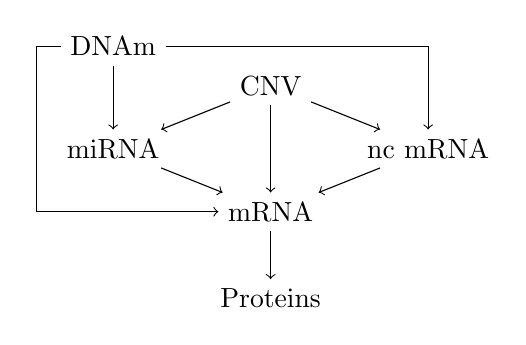
\begin{tikzpicture}<disable externalization>
             \node (DNAm) at (-2,0.5) {DNAm};
             \node (miRNA) at (-2,-0.8) {miRNA};
             \node (CNV) at (0,0) {CNV};
             \node (nc mRNA) at (2,-0.8) {nc mRNA};
             \node (mRNA) at (0,-1.6) {mRNA};
             \node (Proteins) at (0,-2.7) {Proteins};

             \draw [->] (DNAm) to (miRNA);
             \node (temp) at ([xshift=-3mm]DNAm.west) {};
             \draw [->] (DNAm.west) -- (temp.center) |- (temp.center |- mRNA.west) -- (mRNA.west);
             \draw[->] (DNAm) -- node {} ++(2cm,0) -| (nc mRNA);
             \draw [->] (CNV) to (mRNA);
             \draw [->] (mRNA) to (Proteins);
             \draw [->] (miRNA) to (mRNA);
             \draw [->] (nc mRNA) to (mRNA);
             \draw [->] (CNV) to (miRNA);
             \draw [->] (CNV) to (nc mRNA);

         \end{tikzpicture}
         \caption{Interaction graph between modalities used for TCGA}\label{fig:tcga_graph}
     \end{wrapfigure}
     We used the modality interaction graph described in~\cref{fig:tcga_graph} to train CrossAttOmics on TCGA data.
     The details of the different architectures and training hyperparameters is available in~\cref{chap:crossattomics_appendix} \cref{sec:crossattomics_training_details}.
     Attention based architectures, AttOmics EF, AttOmics IF and CrossAttOmics are impacted by the number of groups.
     We used similar numbers of groups as used in~\cite{AttOmics}.
     All models were trained on an Nvidia GeForce RTX 3090.

     All the architectures cannot be tested with all possible combinations due to hardware constraints (see below) or architecture limitations.
     For architecture based on knowledge, not all modalities can be mapped to the knowledge source, for instance miRNA cannot be associated to the \gls{ppi} graph.
     Main results are presented on TCGA, similar results are available for CCLE in~\cref{chap:crossattomics_appendix}.

\section{Results}

 \subsection{Omics combination}
    \begin{figure}[htbp]
        \centering
        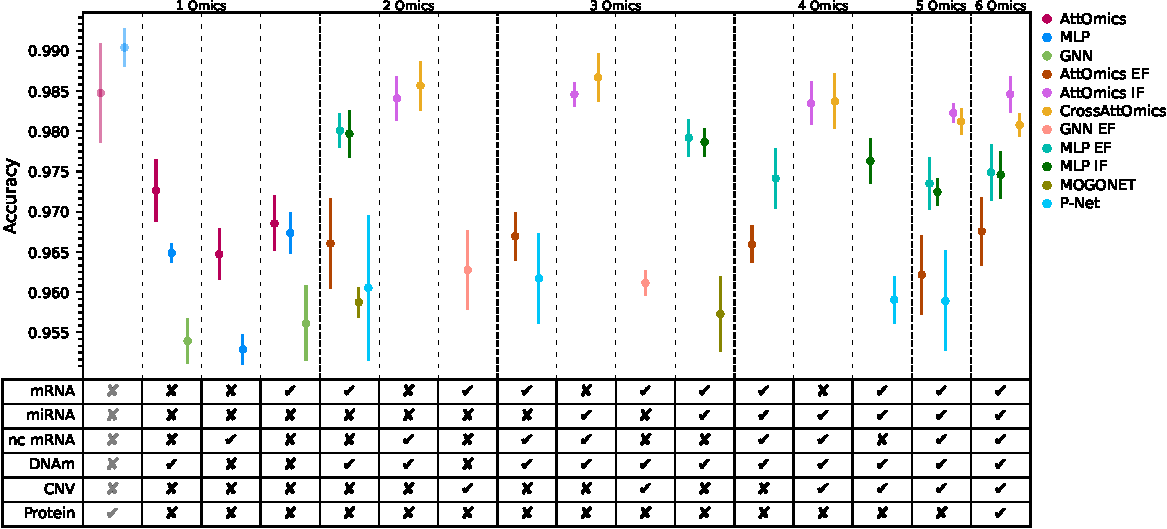
\includegraphics[width=1\textwidth]{tcga_perf_omics_comb.pdf}
        \caption{Comparison of the test accuracy of different multi-omics deep learning integration models across different omics combination on the TCGA dataset. Each dot represents the mean accuracy obtained by a model on the test set after 5 different training. The error-bars represents the standard-error. For each combination a \cmark means that the omics is included in the combination and a \xmark means that the omics is excluded from the combination.}
        \label{fig:tcga_perf_comb}
    \end{figure}
     \Cref{fig:tcga_perf_comb} shows the average and standard deviation of the accuracy on the cancer-type classification task according to the best omics combination for all tested methods on the TCGA dataset.

     For single-omics baselines, \gls{mlp} and AttOmics achieve better performances than the \gls{gnn}.
     Results vary according to the studied omics; AttOmics outperforms the \gls{mlp} when analyzing DNAm or nc mRNA and performs similarly for mRNA and proteins~(\cref{fig:tcga_perf_comb}).
     The best accuracy is obtained with the proteins for the \gls{mlp} and AttOmics.
     On this modality, the best model is the \gls{mlp}, as the number of features is reduced (454 features), grouping the features does not offer any computational advantages.
     The proteins used to construct this dataset were pre-selected as known cancer biomarkers.
     Therefore, they have higher predictive power than the other studied omics.
     With their higher predictive power, proteins can cause biases towards this modality.
     During the training phase, modalities will compete with each other, and only a subset of modalities will win~\cite{pmlr-v162-huang22e}.
     Experimentally, we noticed that including proteins would significantly boost predictive performances for some architectures~(\cref{fig:perf_gain_prot}
     ).
     Furthermore, proteomics is not used for diagnosis due to its high cost~\cite{Mundt2023}.
     For those reasons, we decided not to report the best combination that includes proteins in~\cref{fig:tcga_perf_comb}.
     Complete results are available in~\cref{chap:crossattomics_appendix}.

     Increasing the number of omics available during training can boost performances or have little to no effect on test accuracy.
     There is no change in accuracy when going from two to three modalities with MOGONET.
     It is impossible to test this model with a higher number of modalities due to the huge memory requirements of the architecture.
     The VCDN module, used to perform the integration, requires \(C^{2M}\) parameters.
     For 19 classes and four views, this would represent more than 16 billion parameters.
     P-Net did not benefit either from adding more modalities, and it even reduced the performance.
     The combination of DNAm and mRNA has lower performances than the \gls{mlp} on those individual modalities~(\cref{fig:tcga_perf_comb}).
     AttOmics EF did not benefit from multiple modalities; the performance of the DNAm and mRNA combination is similar to AttOmics on mRNA only and lower than AttOmics on DNAm.
     Adding multiple modalities hinders the performance in this case.
     This architecture did not gain from even more modalities; the performances stayed around the same value.
     The number of groups has been increased to accommodate large multi-omics input, but the architecture is known to be impacted negatively with a large number of groups~\cite{AttOmics}.
     When going from single omics to multi-omics, we observe a small accuracy gain for the \gls{gnn} architecture.
     However, the performances were still lower than AttOmics or \gls{mlp} on single omics.

     Knowledge-based methods are not among the best-performing methods.
     Their performance depends on the quality of the knowledge, which can be incomplete or outdated.
     Incorporating knowledge into the architecture may not necessarily improve performance, but it can enhance the interpretability of predictions.

     Surprisingly, for the \gls{mlp}, the integration strategy, early or intermediate, did not impact the performances.
     Those models achieve better accuracy with two omics than some single omics baselines but could not outperform models only trained on the proteins.
     Adding more omics did not improve the performances and even started to degrade the accuracy.
     The addition of omics brings more noise rather than more information.
     With two and three omics, CrossAttOmics is the best-performing model.
     It can achieve similar accuracy to a model trained on proteins with multiple omics that are not proteins.
     Similarly, AttOmics IF is the second-best model.

     When training on the six available omics, AttOmics IF outperforms CrossAttOmics.
     In this case, AttOmics IF has fewer multimodal parameters than CrossAttOmics and is easier to train.

     \begin{figure*}
        \centering
        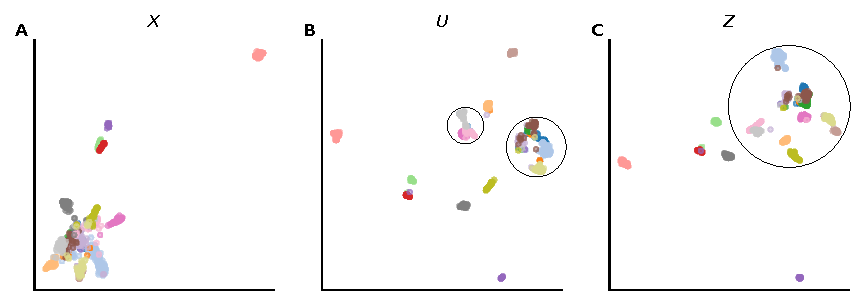
\includegraphics{umap_mRNA.pdf}
        \caption{UMAP comparison of pan-cancer samples in the data space (\textbf{A}), after passing through the modality encoder (\textbf{B}) and after applying the cross-attention (\textbf{C}). Each color represent one of the 18 cancer. }
        \label{fig:umap_mrna}
    \end{figure*}

     To visualize the segregation capabilities in the raw data space, after encoding individual modalities and after enriching individual representation with multi-omics information, we reduce the dimension of each patient representation to a 2D space using a UMAP reduction~(\cref{fig:umap_mrna}).
     Embedding modalities in a latent space with modalities-specific encoders allow for clear identification of cancer clusters, but the separation between some clusters is still unclear (\cref{fig:umap_mrna}A-B).
     The addition of multi-omics information through cross-attention allows better distinguishing the different cancer type-associated clusters (\cref{fig:umap_mrna}C).
     The multi-omics embedding can better represent samples from distinct cancers.


     Given the quadratic complexity of the attention mechanism, we conducted a comparative analysis of the latency, defined as the time required to obtain a prediction from a single sample, across the various multi-omics architectures considered in this study (\cref{fig:latency}).
     It was observed that, for all architectures, an increase in the number of modalities increased the models' latency.
     The CrossAttOmics architecture exhibited the highest latency, which can be attributed to its extensive use of attention mechanisms. Nevertheless, the latency remained reasonable,  a few dozen milliseconds.


     \begin{figure*}[htbp]
         \centering
         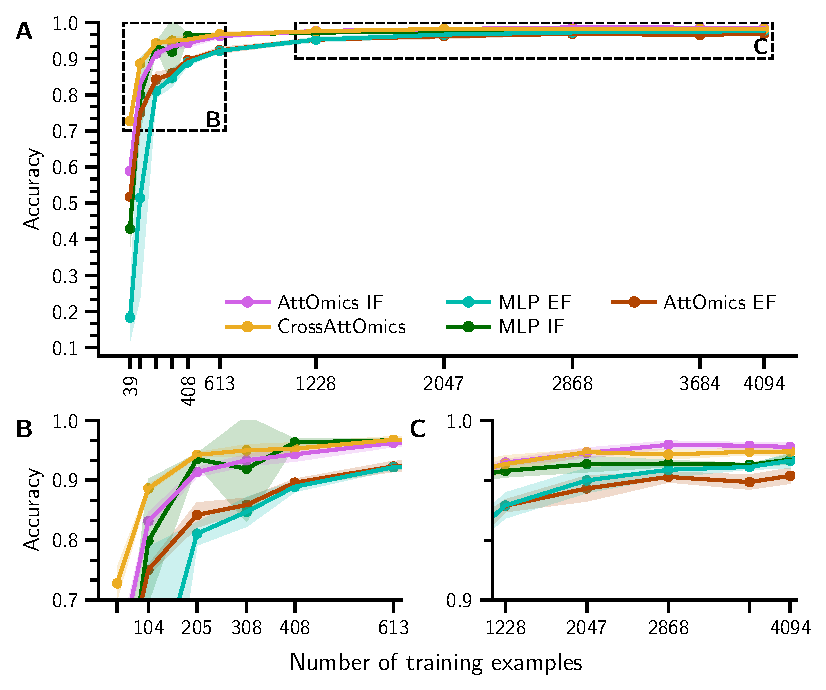
\includegraphics{limited_training_6_omics.pdf}
         \caption{Accuracy on the TCGA test set according to the size of the training set for various multi-omics deep learning models when trained on 6 omics.}
         \label{fig:lim_train_6_omics}
     \end{figure*}
 \subsection{Training with small sample sizes}
     Despite the broad adoption of high throughput methods in personalized medicine, the availability of paired multi-omics data from cancer patients remains limited.
     Many datasets contain partial multi-omics data, where some modalities are entirely missing.
     Modalities missingness is often the result of economic constraints, experimental limitations, or patient refusal~\cite{Kang2021}.
     We explore the impact of the training database size on the performances of CrossAttOmics and other deep-learning architectures by training the different models on a subset of the training set.
     The different subsets are created by randomly sampling 1\%, 2.5\%, 5\%, 7.5\%, 10\%, 15\%, 30\%, 50\%, 70\% and 90\% of the training set while preserving class proportions.
     For each subset, five models are trained.
     The reported performance metrics are estimated on the test set.

     \Cref{fig:lim_train_6_omics} shows the average and standard deviation of the accuracy on the cancer-type classification task according to the training set size for all tested methods on the TCGA dataset.
     The best accuracy is achieved with the highest number of samples.
     Reducing the number of training examples affects model performance adversely, as a limited training database hinders the capacity of the model to extract hidden information during training.

     We observe significant differences between models' accuracy when training with minimal training datasets.
     The MLP EF and AttOmics EF are models sensitive to the size of the training set.
     Despite being easy to implement, early fusion approaches are size-sensitive.
     On the contrary, the intermediate fusion approach is more resistant to small training sets.
     Models' accuracy is lower than those trained on the complete datasets but outperforms early fusion models when trained with less than 600 training examples~(\cref{fig:lim_train_6_omics}B).
     When trained with less than 300 training examples, CrossAttOmics achieves the best accuracy.
     Despite CrossAttOmics and AttOmics IF sharing the same encoder, when trained with only 39 examples, CrossAttOmics outperforms AttOmics IF by more than 0.1 points of accuracy.
     Under limited training settings, cross-attention can improve multimodal representation by allowing modalities to interact and exchange information\footnote{We ran the same experiment using the three best omics for each architecture (\cref{fig:lim_train_3_omics})}.

 \subsection{Robustness to missing modality}
     As mentioned earlier, missing modalities in multi-omics is a challenge.
     We circumvent this problem by narrowing our dataset to only complete multi-omics samples for the training step.
     However, in real-world inference scenarios, it is not feasible to exclude patients simply because of incomplete data.
     The model needs to be robust to different missingness patterns.
     Although machine learning usually deals with missing data by imputing them, omics artificial generation is still challenging.

     A straightforward strategy is to create different missingness patterns during the training~\cite{Cheerla2019}.
     At each iteration, we randomly drop each modality with probability \(P\).
     The maximum number of modalities that can be dropped is a model hyperparameter.

     \Cref{fig:modality_dropout} shows the accuracy distribution with different numbers of missing omics under standard and modality dropout training strategies.
     Each boxplot is calculated with all possible missingness patterns.

     \begin{figure}[htbp]
         \centering
         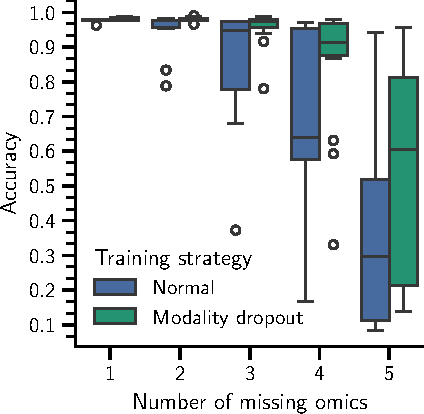
\includegraphics{robustness_missing_modalities_dropout.pdf}
         \caption{Comparison of CrossAttOmics robustness to missing modalities under two different training strategy: classical training and modality dropout. With modality dropout various scheme of missingness are created during training.}
         \label{fig:modality_dropout}
     \end{figure}

     With classical training, increasing the number of missing omics degrades the performance.
     CrossAttOmics is robust to 1 or 2 missing omics, as the multiple cross-attention allows the exchange of information before constructing the multimodal representation.
     With modality dropout, the robustness is increased, and CrossAttOmics can support up to three missing omics without impacting the accuracy.
     The performance is slightly impacted when four omics are missing.
     The impact on the accuracy depends on the omics that are missing.
     The absence of CNV, an uninformative omic, does not have the same impact as the absence of mRNA, an informative omic.
     If many of the most informative omics are missing, the model will not be able to restore the missing information from the less informative omics, even by training the model on this specific missingness pattern.

     Modality dropout is a simple but effective strategy to increase model robustness to missing modalities.

 \subsection{Interaction importances}
     Using gradient-based methods to backpropagate the output in the model, we can identify the most significant interactions.
     One such method is \gls{lrp}.
     \Gls{lrp} aims to back-propagate the prediction signal \(p_c\) in the neural network to assign a relevance score to each neuron.
     We measure the importance of modality interactions as the mean of the \gls{lrp} importance scores assigned to the cross-attention output neurons.

     \begin{wrapfigure}[16]{o}{0.48\textwidth}
        \centering
        \vspace{-\intextsep}
        \begin{tikzpicture}
            \begin{axis}[
            xbar=0pt, bar width=__LRPBARWIDTH__,
            ytick=data, 
            yticklabels from table={\LRPCrossAttOmicsSubset}{cancer}, 
            yticklabel style={rotate=90, font=\footnotesize},
            xticklabel style={font=\scriptsize},
            xlabel style={font=\scriptsize},
            xlabel near ticks,
            xlabel shift=-1mm,
            y dir=reverse, 
            xmin=-0.025,
            xlabel=LRP relevance score, 
            minor x tick num=2, 
            ytick style={draw=none}, ytick align=inside, 
            y axis line style={draw=none},
            xtick pos=lower,
            axis y line*=none,
            axis x line*=bottom,
            height=__LRPHEIGHT__,
            width=__LRPWIDTH__,
            legend to name={LRPsubset},
            legend columns=3,
            enlarge y limits=0.3,
            enlarge x limits=false,
            legend cell align={left},
            legend style={draw=none, row sep=0pt, /tikz/every even column/.append style={column sep=3pt}, font=\tiny,},
                legend image code/.code={%
                     \draw[#1] (0cm,-0.1cm) rectangle (0.3cm,0.1cm);
                }
            ]
                \pgfplotstableforeachcolumn\LRPCrossAttOmicsSubset\as\col{%
            \IfStrEq{\col}{cancer}{}{
                \intCaseF {\pgfplotstablecol} {
                  {9}{
                  \addplot[draw=none,fill=lrp1] table[y expr=\coordindex, x=\col]{\LRPCrossAttOmicsSubset};
                  }
                  {8}{
                  \addplot[draw=none,fill=lrp2] table[y expr=\coordindex, x=\col]{\LRPCrossAttOmicsSubset};
                  %\addlegendentryexpanded{Test2}
                  }
                  {7}{\addplot[draw=none,fill=lrp3] table[y expr=\coordindex, x=\col]{\LRPCrossAttOmicsSubset};}
                  {6}{\addplot[draw=none,fill=lrp4] table[y expr=\coordindex, x=\col]{\LRPCrossAttOmicsSubset};}
                  {5}{\addplot[draw=none,fill=lrp5] table[y expr=\coordindex, x=\col]{\LRPCrossAttOmicsSubset};}
                  {4}{\addplot[draw=none,fill=lrp6] table[y expr=\coordindex, x=\col]{\LRPCrossAttOmicsSubset};}
                  {3}{\addplot[draw=none,fill=lrp7] table[y expr=\coordindex, x=\col]{\LRPCrossAttOmicsSubset};}
                  {2}{\addplot[draw=none,fill=lrp8] table[y expr=\coordindex, x=\col]{\LRPCrossAttOmicsSubset};}
                  {1}{\addplot[draw=none,fill=lrp9] table[y expr=\coordindex, x=\col]{\LRPCrossAttOmicsSubset};}
                }{}
                \verbtocs{\myarrow}|→|
                \StrSubstitute{\col}{---}{→}[\lgdentry]%\textrightarrow
                \addlegendentryexpanded{\lgdentry}
            }
            }
            \end{axis}
            \node[anchor=north, yshift=1ex] at (current axis.below south) {\pgfplotslegendfromname{LRPsubset}};
        \end{tikzpicture}
        %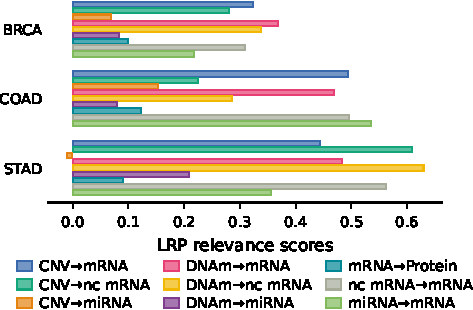
\includegraphics[width=\linewidth]{LRP_crossattomics_subset.pdf}
        \caption{Comparison of the \gls{lrp} relevance score for the different modelled modality interactions for three cancer.}\label{fig:LRP_CrossAttOmics_subset}
    \end{wrapfigure}
    \Cref{fig:LRP_CrossAttOmics_subset} presents the \gls{lrp} attribution score for each considered interaction by cancer.
     Each cancer is characterized by a specific set of important interactions, suggesting that the cross-attention can learn interactions specific to each cancer~(\cref{fig:LRP_CrossAttOmics}).
     Among the various cancers, the interaction of CNVs with mRNAs stands out as a significant interaction.
     Combining CNVs and mRNAs makes it possible to exploit their complementarity, and the level of mRNAs confirms the presence of multiple copies of the gene.
     In the case of colorectal cancer (COAD, \cref{fig:LRP_CrossAttOmics_subset}),  the interaction between miRNA and mRNA has been identified as one of the main interactions for this cancer.
     miRNAs play a crucial role in gene regulatory networks by targeting various mRNAs~\cite{Amirkhah2015}.
     In breast cancer (BRCA, \cref{fig:LRP_CrossAttOmics_subset}), DNAm - mRNA, DNAm - nc mRNA, and nc mRNA - mRNA interactions were identified as among the most important.
     Promoter hypomethylation of tumor suppressor genes, such as BRCA1, promotes tumor initiation and progression~\cite{Szyf2004}.
     Promoter hypomethylation can also upregulate \gls{lncrna}, such as EPIC1, which promotes breast cancer tumourigenesis~\cite{Wang2018}.
     In gastric cancer (STAD, \cref{fig:LRP_CrossAttOmics_subset}), main interactions involve non-coding mRNAs.
     For this cancer, \glspl{lncrna} are known to play key roles in gastric tumourigenesis~\cite{Tan2020}.

\section{Conclusions}
 In this paper, we propose CrossAttOmics, a novel deep-learning approach to combine multi-omics data.
 CrossAttOmics harnesses cross-attention to build a multimodal representation that explicitly considers interactions between modalities.
 While unimodal models trained on specific features, such as proteins in TCGA, can achieve high accuracy, obtaining these features can be challenging and expensive.
 We show that by using only two or three non-protein omics combinations, CrossAttOmics can achieve similar accuracy to that obtained by training only on proteins.
 CrossAttOmics outperforms other deep learning architectures when there are very few paired training examples.
 This is achieved by allowing information to flow between the different omics through the cross-attention layers.
 By explicitly modeling the interactions between different omics, attribution methods such as \gls{lrp} can help in identifying the most important interactions.

 We adopted a two phase training strategy, where modalities encoders are trained independently on the prediction task in a first phase.
 In a second phase the multimodal part, i.e. the fusion through the different cross-attention and the predictor module are trained.
 There are no restrictions on training the model in an end-to-end fashion, it should be noted that this will increase the training time.

 In this work, we only considered omics modalities, but in precision medicine, a wide range of non-omics modalities are available, such as scanners, MRIs, histology slides, or health records.
 The flexible modeling capabilities of the attention mechanism could help develop a multimodal model integrating heterogeneous and complex modalities.

 To assess the significance of modalities interactions, we used post-hoc techniques applied after model training.
 The generated explanations may not fully capture the underlying complexity of the model, and the explanations may not be reliable.
 CrossAttOmics could be improved by integrating trainable weights in the architecture to measure the importance of modalities interactions.


\end{document}
